\documentclass[conference]{IEEEtran}
\usepackage{amsmath,amssymb}
\usepackage{graphicx}
\usepackage{booktabs}
\usepackage{multirow}
\usepackage{cite}
\usepackage{url}
\usepackage{balance}

\begin{document}

\title{DNN Mapping Optimization on Spatial Accelerators:\\
Problem Formulation and Algorithm Comparison}

\author{\IEEEauthorblockN{Author Name}
\IEEEauthorblockA{Course Project: Integrated Circuit Engineering Algorithms\\
Code: \url{https://github.com/mcyinsz/EDA-alg-spatial-mapping}}}

\maketitle

\begin{abstract}
Spatial accelerators (e.g., Cerebras WSE, Groq TSP) interconnect thousands of cores in a 2D mesh. Deploying deep neural networks requires joint \emph{partitioning} (cores per layer) and \emph{placement} (physical mesh positions), a combinatorial optimization problem. We formulate latency minimization with an analytical cost model covering compute, inter-layer, and intra-layer tensor-parallel communication. Four solvers---integer linear programming (ILP), simulated annealing (SA), nested evolution strategy (EA), and Greedy+Kernighan-Lin (Greedy+KL)---are compared on 19 feasible configurations (7 DNN workloads $\times$ 3 mesh sizes). Our key finding: \textbf{problem modeling decisively affects algorithm ranking}. With inter-layer communication only, SA wins 12/19; adding intra-layer communication shifts Greedy+KL to 17/19 wins due to its compact contiguous placement.
\end{abstract}

\section{Introduction}
Spatial architectures place compute and memory on a 2D mesh connected by a network-on-chip (NoC). Inference latency depends not only on the model but on how layers are mapped onto cores. Two coupled sub-problems arise: (i)~\textbf{partitioning}---how many cores each layer uses, trading parallelism for communication; and (ii)~\textbf{placement}---where those cores sit on the mesh, affecting Manhattan routing distance. The search space grows combinatorially: for a 10-layer network on a 152-core chip, partitioning alone exceeds $10^{13}$ choices~\cite{wever2026}.

Prior mapping tools (Timeloop~\cite{parashar2019}, GAMMA~\cite{kao2020}, DiGAMMA~\cite{kao2022}) target hierarchical memory accelerators rather than mesh NoC distance. Wever et al.~\cite{wever2026} use evolutionary search with hardware-in-the-loop on Loihi~2 but require $\sim$5\,s per evaluation. We contribute: (1)~a unified analytical cost model with intra-layer tensor-parallel communication; (2)~four solvers under a common framework; (3)~systematic comparison revealing that modeling choices dominate algorithm rankings.

\section{Problem Formulation}
\subsection{Model}
A DNN has $L$ layers; layer $i$ has FLOPs $F_i$, weight size $W_i$, and activation size $A_i$. The accelerator is an $H{\times}W$ mesh with $K{=}HW$ homogeneous cores (memory $M$, throughput $P$, link cost $\beta$ per byte-hop).

\subsection{Decision Variables}
\textbf{Partitioning} $\mathbf{x}{=}(x_1,\ldots,x_L)$, $x_i{\in}\mathbb{Z}_+$, cores assigned to layer $i$. \textbf{Placement} $S_i{\subset}\{(r,c)\}$, $|S_i|{=}x_i$, physical core positions.

\subsection{Objective}
Minimize total inference latency:
\begin{equation}
\min_{\mathbf{x},\{S_i\}} T = \sum_{i=1}^{L} T_{\text{comp},i} + \sum_{i=1}^{L-1} T_{\text{inter},i} + \sum_{i=1}^{L} T_{\text{intra},i}
\label{eq:obj}
\end{equation}
where $T_{\text{comp},i} = F_i/(x_i P)$,
$T_{\text{inter},i} = \beta (A_i/x_i)\,\bar{d}_{\text{inter}}(S_i,S_{i+1})$,
and $T_{\text{intra},i} = \beta \kappa_i A_i (1{-}1/x_i)\,\bar{d}_{\text{intra}}(S_i)$ for $x_i{>}1$ (else 0).
Average distances $\bar{d}_{\text{inter}}$ and $\bar{d}_{\text{intra}}$ are pairwise Manhattan means over assigned cores; $\kappa_i{=}1.0$ for linear layers, $0.5$ for convolutions.

\subsection{Constraints}
(C1)~$S_i \cap S_j = \emptyset$ for $i{\neq}j$; (C2)~$(W_i{+}A_i)/x_i \leq M$; (C3)~$x_i \geq 1$. The problem is non-convex, tightly coupled, and combinatorially explosive.

\section{Algorithms}
\subsection{ILP}
Binary variables $z_{i,k}$ assign core $k$ to layer $i$. Inter- and intra-layer distance terms are linearized via auxiliary variables ($O(K^2L)$ total). Due to scale, ILP fixes partitioning greedily and optimizes placement only, with a 60\,s time limit on meshes $\leq$16 cores (PuLP+CBC).

\subsection{Simulated Annealing (SA)}
State $(\mathbf{x},\{S_i\})$. Neighborhood: partition perturbation, placement swap, or joint move. Metropolis acceptance with $T_0{=}100$, $\gamma{=}0.995$, 3000 iterations, 3 runs (best reported).

\subsection{Nested Evolution Strategy (EA)}
Following~\cite{wever2026}: outer ES optimizes partitioning genotype; inner ES optimizes placement permutation with a reordering operator preserving spatial locality. $(1{+}\lambda)$ selection with $\lambda{=}4$, 40 generations, 3 runs.

\subsection{Greedy + Kernighan-Lin (Greedy+KL)}
Three phases: (1)~greedy partition by marginal compute benefit; (2)~column-major contiguous placement + KL pair-swap refinement; (3)~single-core partition refinement. Deterministic, one run.

\section{Experimental Results}
\subsection{Setup}
Seven workloads (Small/Medium/Large/Sparse-MLP, Transformer-S/L, ConvNet) on 4$\times$4, 6$\times$6, 8$\times$8 meshes ($M{=}512$\,KB, $P{=}64$ FLOP/cycle, $\beta{=}1.0$). Large-MLP and Transformer-L are infeasible on 4$\times$4 (19 configs total). Five baseline heuristics included. Latencies in $\mu$s at 1\,GHz (relative comparison only). Full reproduction: see repository link in author block.

\subsection{Main Results}
Table~\ref{tab:main} reports best latency ($\mu$s) per solver; bold = best per config. Greedy+KL wins 17/19; SA wins ConvNet/4$\times$4 only; EA wins Small-MLP/4$\times$4; ILP wins none.

\begin{table*}[t]
\centering
\caption{Best inference latency ($\mu$s) per configuration. ``---'': ILP not run ($>$16 cores).}
\label{tab:main}
\scriptsize
\setlength{\tabcolsep}{2.5pt}
\begin{tabular}{lrrrrr}
\toprule
Configuration & Baseline & ILP & SA & EA & Greedy+KL \\
\midrule
Small-MLP/4$\times$4   & 3.84 & 4.66 & 3.78 & \textbf{3.33} & 3.75 \\
Small-MLP/6$\times$6   & 3.84 & ---  & 5.26 & 4.98 & \textbf{4.97} \\
Small-MLP/8$\times$8   & 3.84 & ---  & 7.17 & 8.17 & \textbf{6.68} \\
Medium-MLP/4$\times$4  & 27.1 & 26.9 & 25.4 & 25.5 & \textbf{25.2} \\
Medium-MLP/6$\times$6  & 29.3 & ---  & 29.4 & 30.7 & \textbf{28.2} \\
Medium-MLP/8$\times$8  & 32.3 & ---  & 39.4 & 41.0 & \textbf{29.5} \\
Large-MLP/6$\times$6   & 44.7 & ---  & 45.0 & 48.2 & \textbf{38.1} \\
Large-MLP/8$\times$8   & 47.2 & ---  & 57.4 & 60.2 & \textbf{43.1} \\
Sparse-MLP/4$\times$4  & 21.8 & 22.3 & 20.7 & 21.2 & \textbf{20.6} \\
Sparse-MLP/6$\times$6  & 26.2 & ---  & 27.6 & 29.3 & \textbf{25.6} \\
Sparse-MLP/8$\times$8  & 24.6 & ---  & 37.0 & 39.8 & \textbf{28.3} \\
Transformer-S/4$\times$4 & 23.2 & 21.4 & 20.9 & 21.3 & \textbf{19.8} \\
Transformer-S/6$\times$6 & 21.9 & ---  & 24.8 & 27.0 & \textbf{19.7} \\
Transformer-S/8$\times$8 & 24.6 & ---  & 34.5 & 33.5 & \textbf{21.3} \\
Transformer-L/6$\times$6 & 57.7 & ---  & 62.6 & 61.8 & \textbf{46.8} \\
Transformer-L/8$\times$8 & 68.7 & ---  & 74.0 & 74.6 & \textbf{46.8} \\
ConvNet/4$\times$4      & 859  & 826  & \textbf{810} & 816 & 813 \\
ConvNet/6$\times$6      & 838  & ---  & 826  & 889 & \textbf{764} \\
ConvNet/8$\times$8      & 937  & ---  & 1010 & 1105 & \textbf{848} \\
\bottomrule
\end{tabular}
\end{table*}

\subsection{Analysis}
Fig.~\ref{fig:heatmap} shows normalized latency (best$=$1.0). Greedy+KL dominates on large meshes where intra-layer distance penalties are severe (e.g., Transformer-L/8$\times$8: 46.8 vs.\ SA 74.0\,$\mu$s, $-$37\%). Fig.~\ref{fig:breakdown} decomposes latency: Greedy+KL keeps intra-layer share $<$15\% via compact clusters; SA/EA reach 20--40\% due to fragmented placement. Fig.~\ref{fig:mapping} illustrates Greedy+KL's symmetric partitioning on Large-MLP/8$\times$8. Fig.~\ref{fig:wins} confirms dominance across MLP, Transformer, and ConvNet families.

\begin{figure}[!t]
\centering
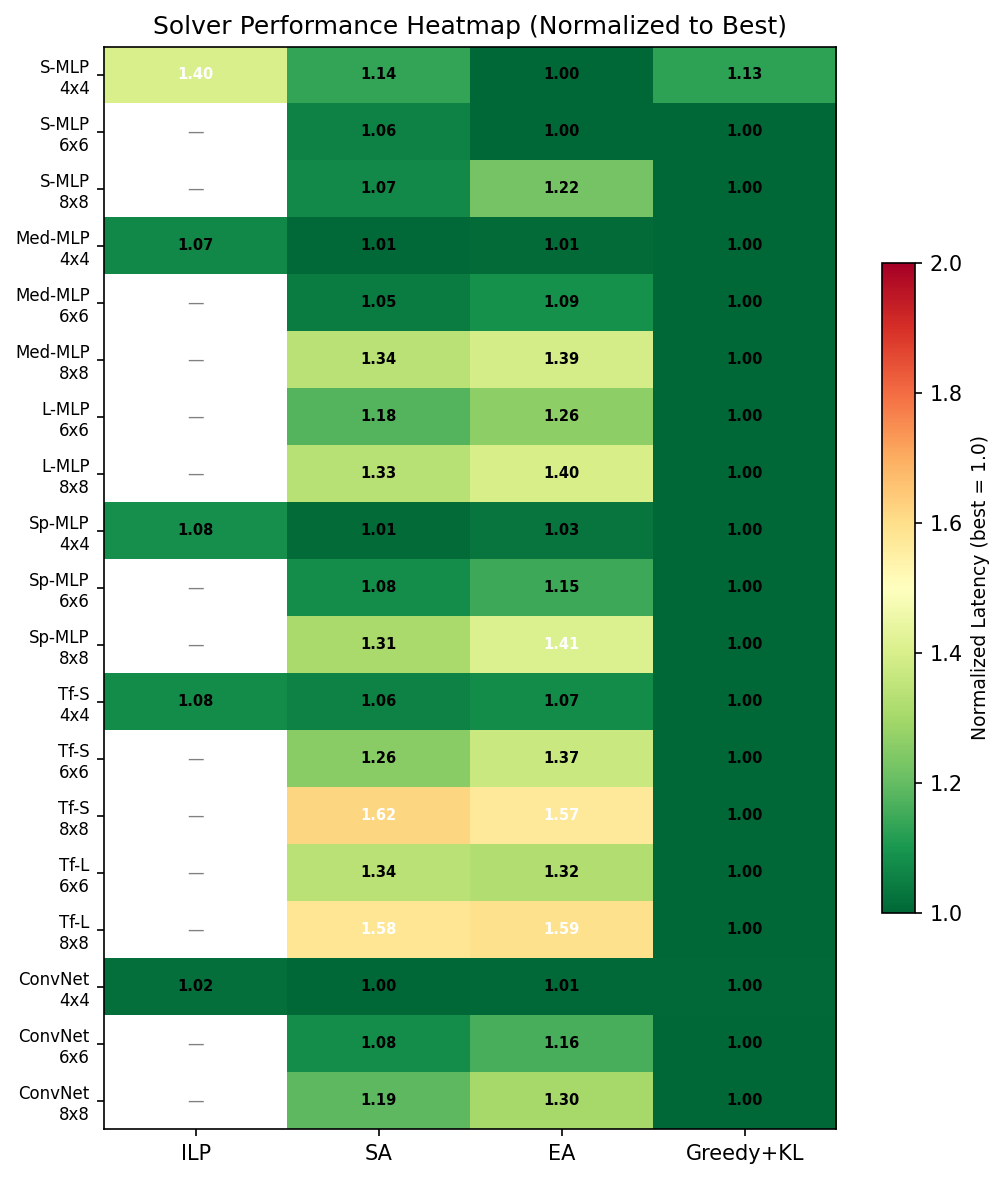
\includegraphics[width=\linewidth]{../results/normalized_heatmap.png}
\caption{Normalized latency heatmap (best solver $=$ 1.0 per config).}
\label{fig:heatmap}
\end{figure}

\begin{figure}[!t]
\centering
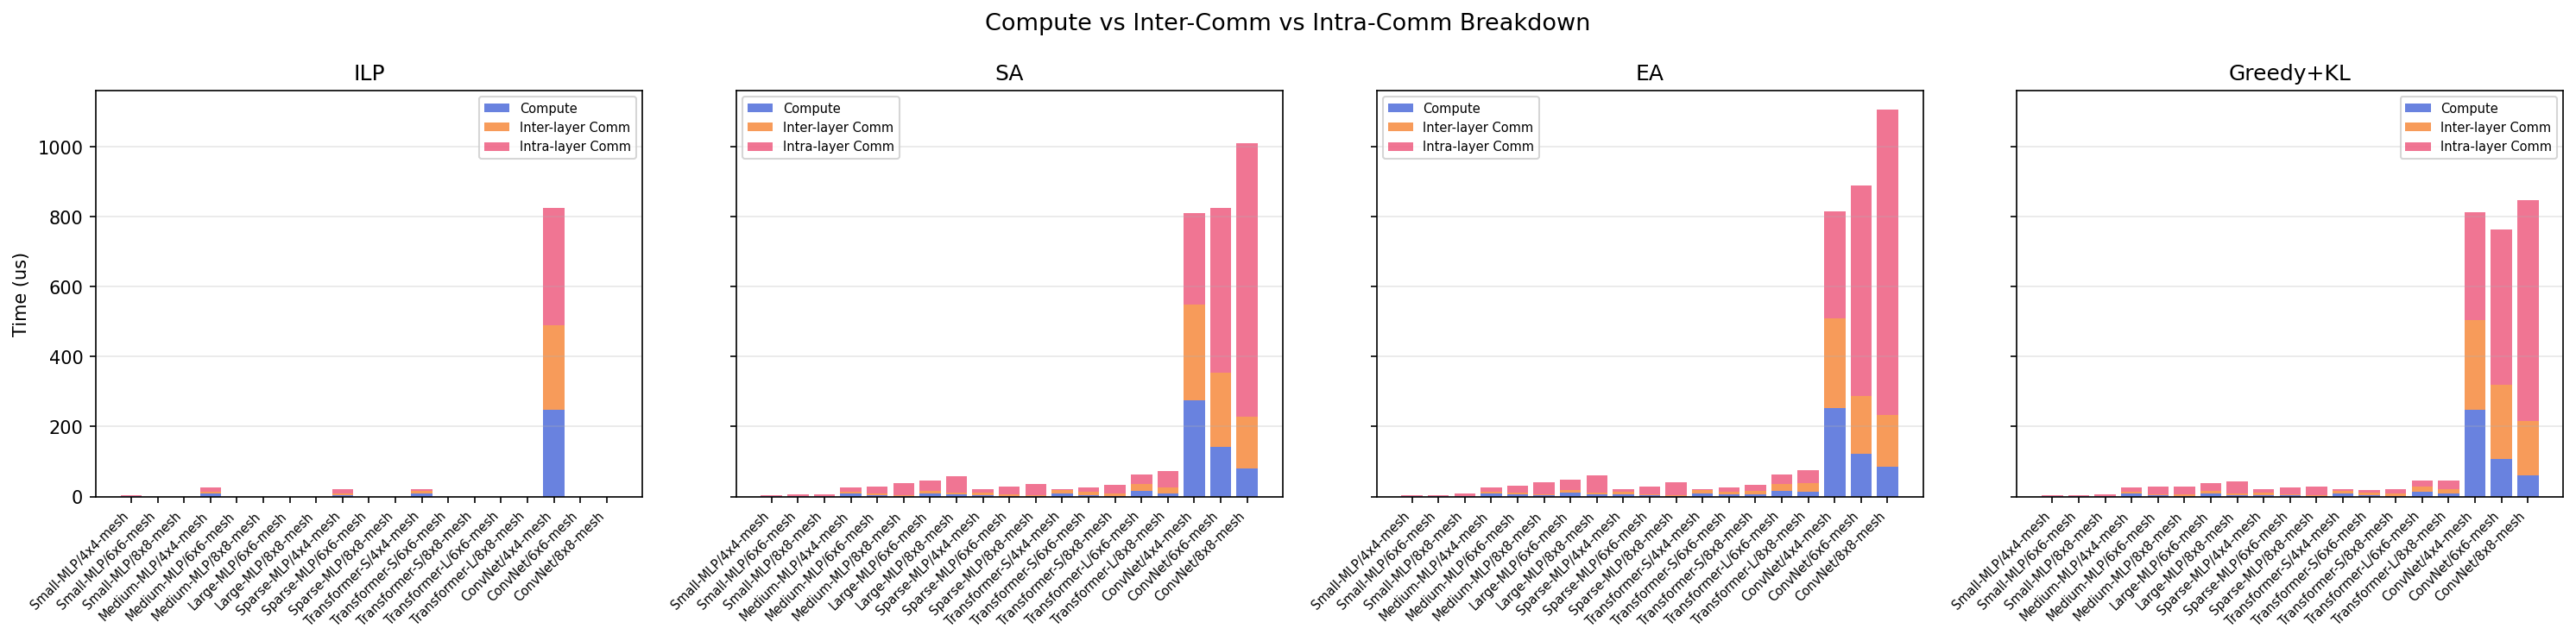
\includegraphics[width=\linewidth]{../results/compute_comm_breakdown.png}
\caption{Compute, inter-layer, and intra-layer latency breakdown.}
\label{fig:breakdown}
\end{figure}

\begin{figure}[!t]
\centering
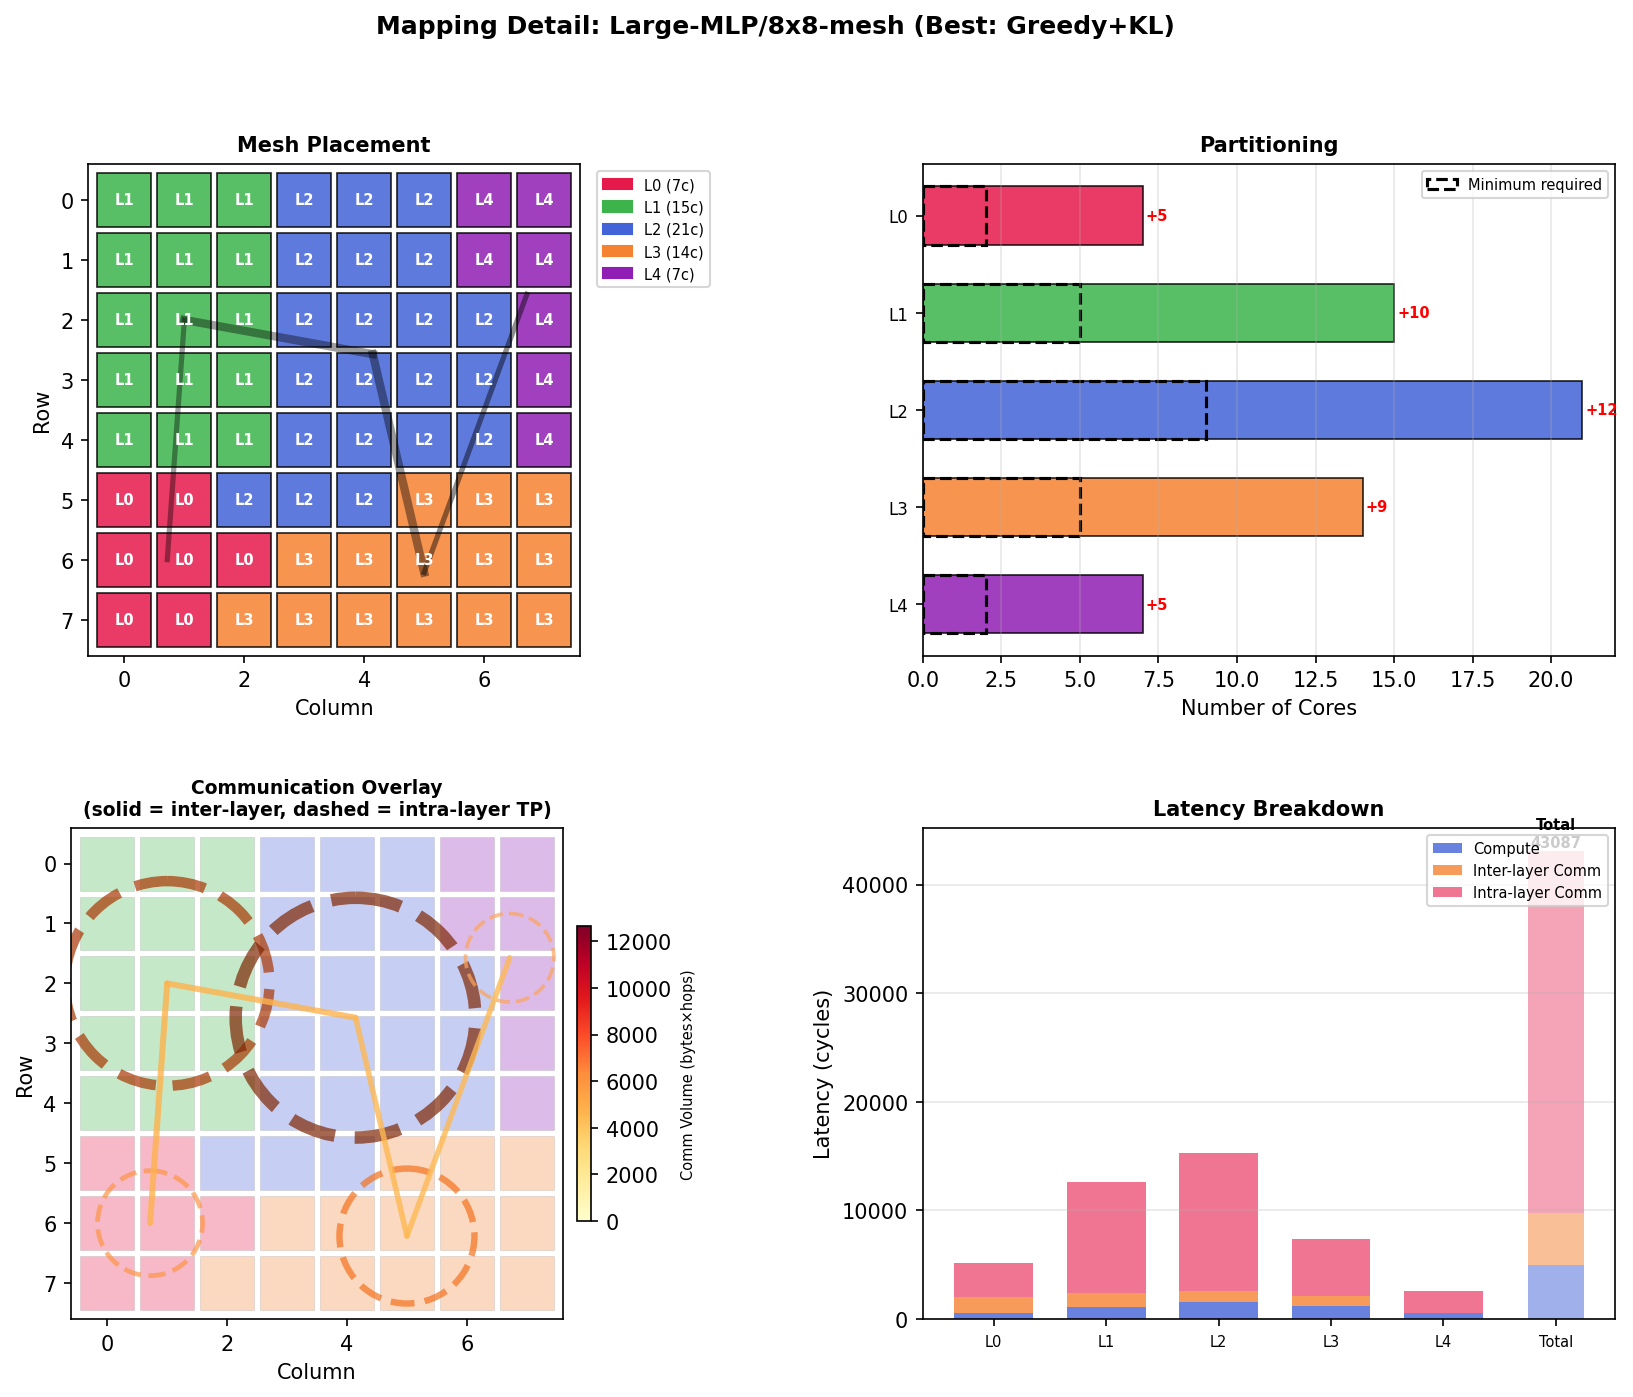
\includegraphics[width=\linewidth]{../results/mapping_detail_Large-MLP_8x8-mesh.png}
\caption{Greedy+KL mapping for Large-MLP/8$\times$8 (43.1\,$\mu$s).}
\label{fig:mapping}
\end{figure}

\begin{figure}[!t]
\centering
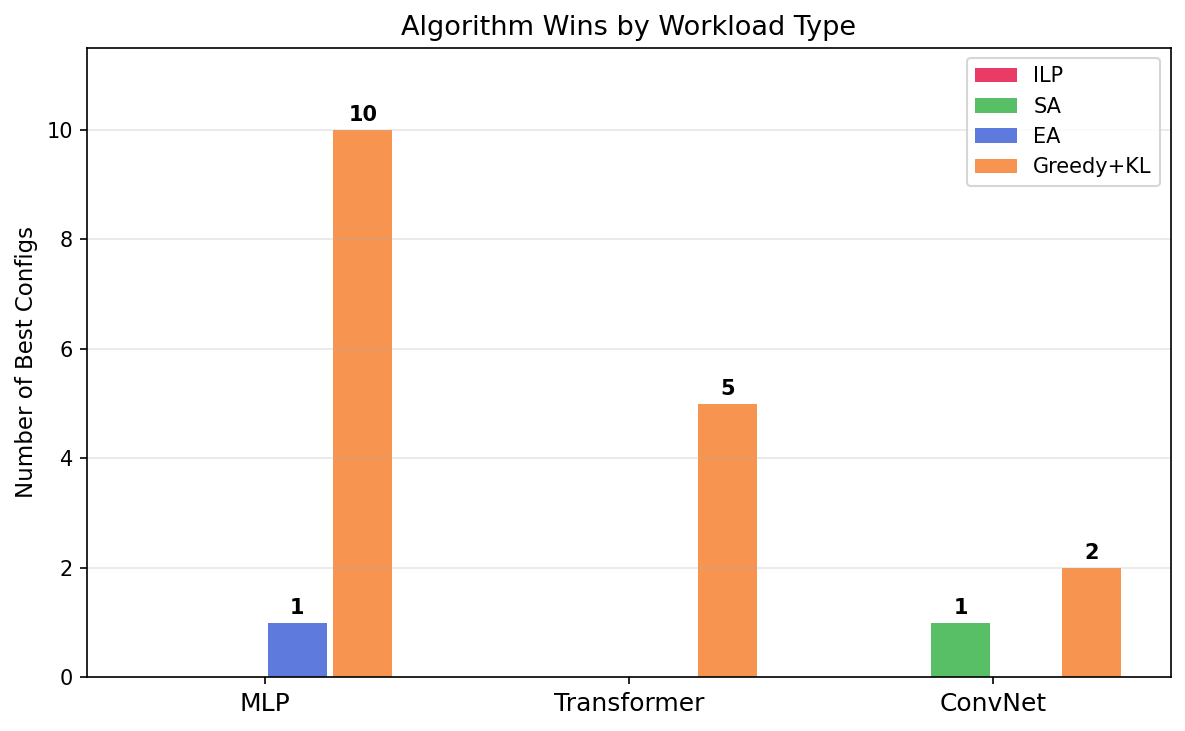
\includegraphics[width=\linewidth]{../results/algorithm_wins_by_type.png}
\caption{Number of configurations where each solver achieves best latency.}
\label{fig:wins}
\end{figure}

With \emph{inter-layer communication only} (ablation), SA wins 12/19---demonstrating that intra-layer modeling reverses rankings. SA retains a marginal edge on ConvNet/4$\times$4 where mesh is small and intra-layer penalty is limited.

\section{Conclusion}
We formulated DNN mapping on spatial accelerators as joint partitioning-placement optimization with a three-term latency model. Greedy+KL's contiguous placement aligns with intra-layer communication costs, yielding 17/19 wins. SA's random-swap neighborhoods degrade on large meshes; ILP is limited by fixed partitioning and quadratic variable growth. Future work: block-move neighborhoods for SA/EA, surrogate models, and validation on real hardware.

\begin{thebibliography}{00}
\bibitem{yik2025} J.~Yik \textit{et al.}, ``Modeling and optimizing performance bottlenecks for neuromorphic accelerators,'' arXiv:2511.21549, 2025.
\bibitem{timcheck2026} J.~Timcheck \textit{et al.}, ``A compute and communication runtime model for Loihi~2,'' arXiv:2601.10035, 2026.
\bibitem{wever2026} M.~Wever \textit{et al.}, ``Evolutionary mapping of neural networks to spatial accelerators,'' arXiv:2602.04717, 2026.
\bibitem{parashar2019} A.~Parashar \textit{et al.}, ``Timeloop: A systematic approach to DNN accelerator evaluation,'' in \textit{ISPASS}, 2019, pp.~304--315.
\bibitem{kao2020} S.~Kao and T.~Krishna, ``GAMMA: Automating the HW mapping of DNN models on accelerators via genetic algorithm,'' in \textit{ICCAD}, 2020, pp.~1--9.
\bibitem{kao2022} S.~Kao \textit{et al.}, ``DiGAMMA: Domain-aware genetic algorithm for HW-mapping co-optimization,'' in \textit{DATE}, 2022, pp.~232--237.
\bibitem{lie2024} S.~Lie, ``Inside the Cerebras wafer-scale cluster,'' \textit{IEEE Micro}, 2024.
\bibitem{abts2020} D.~Abts \textit{et al.}, ``Think fast: A tensor streaming processor for accelerating deep learning workloads,'' in \textit{ISCA}, 2020.
\end{thebibliography}

\balance
\end{document}
